\documentclass[14pt,a4paper,oneside]{extarticle}
\usepackage{amsmath}\usepackage{amsfonts}\usepackage{amssymb}\usepackage{pgfplots}
\usepackage{setspace}\usepackage{mathtools}\usepackage{tikz}\usetikzlibrary{arrows}

\usepackage[utf8]{inputenc}\usepackage[english, russian]{babel}\usepackage[T2A]{fontenc}\usepackage{enumitem}

\makeatletter\AddEnumerateCounter{\asbuk}{\russian@alph}{щ}\makeatother
\DeclareMathOperator{\sinc}{sinc}\pgfplotsset{compat=1.18}\usepackage{setspace}
% \onehalfspacing
\newcommand{\tb}[1]{\textbf{#1}}
\newcommand{\pic}{\[\tb{Картинка}\]}
\newcommand{\fo}{\[\tb{Формула}\]}
\usepackage{tikz}
\usetikzlibrary{shapes.geometric,shapes.arrows,decorations.pathmorphing}
\usetikzlibrary{matrix,chains,scopes,positioning,arrows,fit, automata}
\usepackage{bookmark}
\usepackage{blindtext}
% \setcounter{secnumdepth}{0}
\usepackage{graphicx}
\graphicspath{ {./images/} }
\usepackage{relsize}
\usepackage{indentfirst}
\usepackage{icomma}

\hyphenpenalty=10000
% \sectionfont{\normalsize}
% \subsectionfont{\normalsize}
% \subsubsectionfont{\normalsize}
% \paragraphfont{\normalsize}
\usepackage{float}
\usepackage{amsthm}

% ГОСТовские настройки для полей и абзацев
\usepackage[a4paper, left=30mm,right=15mm,top=20mm,bottom=20mm]{geometry}
\usepackage{misccorr}
\usepackage{indentfirst}
\usepackage{enumitem}
\setlength{\parindent}{1.25cm}
\linespread{1.5}
\setlist{nolistsep} % Отсутствие отступов между элементами \enumerate и \itemize

% Переопределение стандартных \section, \subsection, \subsubsection по ГОСТу;
% Переопределение их отступов до и после для 1.5 интервала во всем документе
\usepackage{titlesec}
%Если захочется шрифт жирным сделать в секциях \bfseries
%\titleformat{\chapter}[block]
%{\normalsize\bfseries\center}{}{0pt}{}

\titleformat{\section}[block]
{\normalsize\bfseries}{\thesection}{1em}{}
\titlespacing\section{\parindent}{*4}{14pt}

\titleformat{\subsection}[hang]
{\normalsize\bfseries}{\thesubsection}{1em}{}
\titlespacing\subsection{\parindent}{*4}{14pt}
%\titlespacing\subsection{\parindent}{\parskip}{\parskip}

\titleformat{\subsubsection}[hang]
{\normalsize\bfseries }{\thesubsubsection}{1em}{}
\titlespacing\subsubsection{\parindent}{*4}{14pt}
%\titlespacing\subsubsection{\parindent}{\parskip}{\parskip}

\newtheorem*{theorem}{Теорема}
% \makeatletter
% \renewcommand{\@seccntformat}[1]{\csname the#1\endcsname.\quad}
% \makeatother
\hypersetup{%
    pdfborder = {0 0 0}
}

% \fussy
\sloppy

\usepackage{tocloft}
\renewcommand{\cftsecleader}{\cftdotfill{\cftdotsep}} % точки на всех строках
\renewcommand{\cftsecfont}{\normalsize}% titles in bold
\renewcommand{\cftsubsecfont}{\normalsize}% titles in bold
\renewcommand{\cftsubsubsecfont}{\normalsize}% titles in bold
\renewcommand{\cftsecpagefont}{\normalfont} % не жирная нумерация section'ов
\setlength{\cftsubsecindent}{0em}
\setlength{\cftsubsubsecindent}{0em}
\setlength{\cftsecnumwidth}{2em}
\setlength{\cftsubsecnumwidth}{2em}
\setlength{\cftsubsubsecnumwidth}{2em}
\setlength{\cftbeforesecskip}{0em}


%Для нумерованных абзацев
\usepackage{enumerate}
\usepackage{enumitem}
\RequirePackage{calc} %Для складывания чисел
%Нумерация числовых строк по ГОСТ
\renewcommand{\labelenumi}{\arabic{enumi})} %( 1),2),3))
\renewcommand{\labelenumii}{\alph{enumii})} %( a),b),c))
%Интервал между строками как в обычном тексте
%Интервал в itemize
\setlist[itemize,1]{leftmargin=0pt,itemindent=(\parindent+0.5\labelwidth),topsep=0pt,itemsep=0pt,parsep=0pt,partopsep=0pt}
\setlist[itemize,2]{leftmargin=\parindent,itemindent=(\parindent+0.5\labelwidth),topsep=0pt,itemsep=0pt,parsep=0pt,partopsep=0pt}
\setlist[itemize,3]{leftmargin=\parindent,itemindent=(\parindent+0.5\labelwidth),topsep=0pt,itemsep=0pt,parsep=0pt,partopsep=0pt}
%Интервал в enumirate
\setlist[enumerate,1]{leftmargin=0pt,itemindent=(\parindent+0.66\labelwidth),topsep=0pt,itemsep=0pt,parsep=0pt,partopsep=0pt}
\setlist[enumerate,2]{leftmargin=\parindent,itemindent=(\parindent+0.66\labelwidth),topsep=0pt,itemsep=0pt,parsep=0pt,partopsep=0pt}
\setlist[enumerate,3]{leftmargin=\parindent,itemindent=(\parindent+0.66\labelwidth),topsep=0pt,itemsep=0pt,parsep=0pt,partopsep=0pt}


\begin{document}
\global\hbadness=10000

\begin{center}
    \renewcommand{\contentsname}{\normalsize\bfseries\centering СОДЕРЖАНИЕ}
    \normalsize
    \tableofcontents
    \normalsize
\end{center}

\pagebreak

\section{Назначение и задачи систем спутниковой связи. Достоинства и недостатки системы спутниковой связи.}

Задачи спутниковой связи, военной и гражданской, ― обеспечение информационной безопасности Российской Федерации.

Назначение: обеспечение связи (радио- и телевещание, телефон, телеграф, передача данных, Интернет, различные приложения ― телеобучение, телемедицина и т.п., функционирование систем обеспечение безопасности Российского государства) ― между любыми территориями на поверхности Земли, а также между территориями, не имеющими общей границы с территорией РФ. В том числе:

\begin{itemize}
    \item районы Крайнего севера, Арктика и Антарктика;
    \item пустыни и высокогорные районы;
    \item поверхность мирового океана с многочисленными островами;
    \item обеспечение связью и мониторинг движения гражданской авиации;
    \item территории, не охваченные другими видами связи;
    \item территории, охваченные другими видами связи.
\end{itemize}

ССС в интересах национальной безопасности Российской Федерации предназначена для обеспечения сбалансированной организации работ по созданию, совершенствованию и интеграции подсистем управления ВС РФ (всех звеньев управления ВС РФ, видов и родов войск ВС, специальных войск), воинскими формированиями и органами, а также Федеральных органов государственной власти и органов власти субъектов РФ в мирное время, в чрезвычайных и кризисных ситуациях, в угрожаемый период и в условиях военного времени (в условиях мирного и военного времени).

Достоинствами спутниковой системы связи являются:

\begin{itemize}
    \item  минимальное время и минимальные затраты, необходимые на наращивание земного (потребительского) сегмента спутниковой связи при существующем космическим сегменте;
    \item возможность организации связи в труднодоступных районах;
    \item широкое покрытие территории космическим РТР орбитальной группировки (ОГ);
    \item возможность организации многостанционного доступа, что позволяет наращивать пропускную способность систем;
    \item возможность организации подвижной связи (в том числе и широкополосной);
    \item простота организации односторонних (вещательных) видов связи (например, спутникового ТВ).
\end{itemize}

Недостатками спутниковой системы связи являются:

\begin{itemize}
    \item высокая стоимость и научно-техническая сложность реализации ССС (например, по сравнению с РРЛС), особенно стоимость и сложность построения космической ОГ;
    \item высокая стоимость услуг и низкая коммерческая эффективность, в основном, за счёт высокой стоимости создания ОГ космических РТР (примеры – Thuraya, Iridium);
    \item необходимость создания высокого энергетического потенциала связи на аппаратах ОГ космических РТР;
    \item более низкая пропускная способность по сравнению с наземными системами связи (ВОЛС, радиорелейная, сотовая);
    \item ограниченность ёмкости орбит, а именно количества точек стояния КА на ГСО.
\end{itemize}

\section{Радиационные пояса Ван-Аллена (Van Allen belt).}

Внутренний пояс находится на высоте от 3 до 12 тыс. км над поверхностью Земли, а внешний – на высоте от 18 до 57 тыс. км. Внутренний состоит главным образом из протонов, а внешний - из электронов.

Разделение на внутренний и внешний пояса достаточно условно, поскольку все околоземное пространство заполнено заряженными частицами, которые движутся в магнитном поле Земли. Наличие радиационных поясов и их характеристики учитываются при проектировании спутников, поскольку длительное пребывание электронной техники в таких условиях чревато поломками.

\section{История развития систем спутниковой связи. Пять характерных этапов развития спутниковой связи.}

\begin{enumerate}
    \item 1957―1965 гг. Подготовительный период…, который начался в октябре 1957 г. запуском Советским Союзом первого в мире ИСЗ Земли, а спустя месяц и второго. Вначале спутниковые информационные технологии создавались, прежде всего, в интересах военных. Этап характеризуется запуском экспериментальных ИСЗ, в том числе КА связи, которые выводились преимущественно на высокоэллиптические (КА Молния-1) и низкие околоземные  орбиты. Первый космический РТР TELSTAR выведен на ГСО в июле 1962 г. в интересах армии США. В тот же период времени была разработана серия американских военных спутников связи SYNСОМ (Synchronous Communications Satellite). К подготовительному периоду относится и создание Международного консорциума спутниковой связи Intelsat (International Telecommunications Satellite Consortium) в 1964 г. с одиннадцатью странами, объединившими технические и финансовые возможности для совместного использования ОГ телекоммуникационных геостационарных КА. Количество стран-участниц постоянно возрастает, и к середине 2006г. её членами уже были 144 страны. Через 24 КА системы Intelsat, размещенных группами над Атлантическим, Индийским и Тихим океанами передается примерно 2/3 международного телефонного трафика стран-участниц и осуществляется почти весь ТВ обмен, а часть стволов сдается в аренду. Космическая группировка обеспечивает глобальное покрытие. Первые КА серии Intelsat обеспечивали трансконтинентальную связь, поддерживая магистральные каналы между небольшим количеством национальных шлюзовых ЗС, обеспечивающих интерфейс с национальными наземными сетями общего пользования, а именно телефонный трафик, ТВ сигналы и телексную связь. Большинство КА размещалось на ГСО, использовался диапазон 6/4 ГГц, а для покрытия возможно большей площади Земли применялись бортовые антенны с широким глобальным лучом. Аппаратура связи и методы передачи были полностью аналоговыми. При передаче аналогового ТВ сигнала для обеспечения высокой помехоустойчивости использовалась частотная модуляция, причем одна телевизионная программа полностью занимала один ствол РТР. РТР, такие как Intelsat-I, -II, -III, представляли собой, по сути, электронные зеркала.
    \item 1965―1973 г.г. Период развития глобальных ССС на основе геостационарных ретрансляторов. Первые два КА серии SYNCOM-3 были запущены на геосинхронные эллиптические орбиты в феврале 1963г. и явились прототипом первого гражданского коммерческого геостационарного КА Intelsat-1 международной организации Intelsat (International Telecommunications Satellite Organization), учрежденной в августе 1964 г. Коммерческие услуги спутниковой связи в этот период ещё не были доступны, но, главное, была экспериментально доказана возможность производства, запуска и успешной работы ССС через КА, базирующихся на околоземной орбите.
    \item 1973―1982 г.г. Этап широкого распространения региональных и  национальных ССС. В течение этого периода достаточно интенсивно разворачивались региональные (Eutelsat, Aussat) и национальные (Skynet, США) ССС,  основными услугами которых по-прежнему были телефония и телевидение, а также в незначительном объеме передача данных. Но теперь эти услуги предоставлялись большому числу наземных абонентских терминалов (АТ), а в некоторых случаях передача осуществлялась непосредственно на  пользовательские АТ. На этом этапе исторического развития ССС была создана  международная организация Inmarsat, развернувшая глобальную сеть связи Inmarsat, основной целью которой было обеспечение связи с морскими судами, находящимися в плавании.
    \item 1982―1990 гг. Период стремительного развития и распространения малых земных абонентских терминалов В 80-е годы успехи в области техники и технологии ключевых элементов ССС позволили использовать спутниковые каналы в корпоративных деловых сетях связи, получивших название VSAT. Там просто пиздец дохуя написано про них, в пизду.
    \item С первой половины 90-х г. ССС вступили в этап использования «интеллектуальных» КА связи. Появилось большое количество глобальных и региональных ССС. Технология спутниковой связи стала областью значительного научного интереса. В этот период времени наблюдался взрывной рост быстродействия микропроцессоров общего назначения и объемов памяти  полупроводниковых устройств при одновременном повышении надежности и уменьшении энергопотребления и стоимости. Микропроцессоры космического применения стали строится радиационно устойчивыми (space military).
\end{enumerate}

\section{Первый кризис системы спутниковой связи. Конкурентная борьба с подводными волоконно-оптическими кабелями. Технические решения, позволившие системе спутниковой связи найти выход из кризиса и определить своё место в глобальной системе инфокоммуникации.}

Развитие ССС происходило в острой конкурентной борьбе с наземными технологиями связи, которая велась с переменным успехом. Такие компании, как Bell Labs, Corning и ряд других, в 80-90-х годах построили крупномасштабные наземные сети ВОЛС.
Первый подводный волоконно-оптический кабель ТАТ-8, проложили через Атлантический океан и соединили США, Великобританию и Францию. Эксплуатация ТАТ-8 началась в 1988 году. За ним быстро последовали ТАТ-9 и 10 (1992г.), ТАТ-11 (1993г.) и ТАТ-12 (1995г.). Не менее быстро росло и число кабелей через Тихий океан.

В направлении «восток$\longleftrightarrow$запад» был проложен кабель, соединивший континентальную часть США (Калифорния), Гавайи, Гуам и  Японию, в направлении «юг$\longleftrightarrow$север» кабели «Гавайи$\longleftrightarrow$Новая Зеландия» и «Гуам$\longleftrightarrow$Австралия».

Использование частотного (по длине волны) мультиплексирования  и промежуточных оптических усилителей-ретрансляторов обеспечило практически неограниченную пропускную способность ВОЛС.
В результате «удельный вес» ССС в мировых технологиях связи заметно снизился. Например, если доля сети Intelsat в поддержке международного телефонного трафика составляла в конце 80-х годов около 70\%, то ко второй половине 90-х годов она упала до 30\% и наблюдалась тенденция к его дальнейшему снижению.
В те же годы телефонные компании были полны оптимизма по поводу решения с помощью ВОЛС проблемы «последней мили».
Прокладка оптических кабелей в каждый дом и квартиру обеспечила бы широкий спектр мультимедийных услуг посредством передачи разнородного трафика по одной физической среде.

Параллельно предлагались альтернативные ВОЛС проекты. Система HALO (High Altitude Long Operation) компании Angel Technologies предполагала использовать специально оборудованные самолеты. Он летает над обслуживаемой территорией на высоте около 15 км по кругу диаметром 4 км, что обеспечивая связью область диаметром 80-120 км.Для круглосуточного обслуживания предполагалось использование посменно 3-х самолетов.

Применение в качестве первичного источника энергии для питания бортовой аппаратуры реактивных двигателей позволяет обеспечить выходную мощность передатчиков около 40 кВт, что без труда решало проблему прохождения радиосигналов Ka диапазона частот через облачный покров и получения пропускной способности каналов до 10 Мбит/с в обоих направлениях.

Наибольший вклад в стоимость ВОЛС вносят затраты на прокладку кабелей и стоимость самого кабеля, поэтому стоимость ВОЛС определяется в первую очередь её протяженностью.
На стоимость наземного магистрального канала  связи влияет также его пропускная способность, число точек подключения к нему пользователей, особенности территории, по которой прокладывается кабель и т.д., но это влияние проявляется намного слабее.

Компания Sky Station предлагала разместить огромную платформу с установленными на ней радиоаппаратурой, двигателями, солнечными батареями и топливными элементами на высоте чуть более 20 км. Поддерживаемая множеством заполненных гелием аэростатов,  платформа должна была занимать геостационарную позицию со сроком службы 5 — 10 лет. Предполагалось обеспечивать передачу информации к пользователям со скоростями до 10 Мбит/с, а в противоположном направлении — 2 Мбит/с.

Все это привело к достаточно широкому распространению среди  специалистов мнения, что ССС прошли пик своего расцвета, а их место в мировой инфо-телекоммуникационной структуре весьма скромно и сводится, в основном, к  вещанию ТВ-программ на головные станции сетей кабельного телевидения и обслуживанию подвижных пользователей.

С другой стороны, в этот же период времени в мире происходили серьёзные политические, технические и экономические события.
Считается, что  основными событиями, предопределившими место и роль ССС, а также области их применения, явились повсеместный рост потребности в телекоммуникационных услугах, особенно в широкополосной передаче данных, что в значительной мере  обусловлено распространением по всему миру услуг сети Интернет и  необходимости скоростного доступа к её информационным ресурсам.
Технические решения и возможности современных космических технологий связи по реализации этих потребностей в 1993 г.  продемонстрировал экспериментальный геостационарный КА ACTS. Появление на рынке компактных и относительно недорогих пользовательских АТ ЗС также ускорило модернизационные процессы сфере спутниковой связи.

И крупные транснациональные фирмы, работающие в   аэрокосмической отрасли военно-промышленного комплекса США,  такие как Hughes, Lockheed Martin, Motorola, Loral, GE-Americom и др., устремились на рынок гражданских коммерческих ССС.

Причем пришли они на этот рынок не с пустыми руками, а  «прихватили» с собой новейшие, еще недавно секретные технологии космической связи, причём не только свои, но и Советского Союза.

Правительство США проявляло все меньше интереса к финансированию развития и модернизации чисто военных ССС, таких как DSCS и КА МО США Milstar, оказывая на МО США определенное давление с целью привлечения его к использованию в своих целях части ресурсов гражданских сетей 40\%  трафика военных сообщений шло через гражданские сети.

Развитие рынка космической связи стимулировала ведущие  мировые аэрокосмические корпорации к обеспечению своей многопрофильности и расширению сферы деятельности, включающей производство бортового и наземного оборудования, спутников, обеспечение запусков,  развертывание наземного сегмента, участие в совместных проектах, провайдерскую деятельность.

По оценкам специалистов, сделанным несколько лет назад, сплошная «кабелизация» при помощи ВОЛС такой, например, страны, как Япония обошлась бы примерно в \$400 млрд. и продолжалась бы более 20 лет, причем существенный вклад в общие затраты внесла бы стоимость работ по прокладке кабелей.

Аналогичная деятельность только в одном штате США Калифорния потребовала бы примерно столько же времени и \$30 млрд., чего вполне хватило для создания, развертывания и поддержания ССС Intelsat, охватывающей  практически весь мир.

В то же время в развивающихся странах усиливаются процессы урбанизации и рост численности городов. Содействие проникновению передовых телекоммуникационных технологий в развивающиеся страны становится долговременной стратегией развития ССС. Одной из особенностей этого развития является возможность полного контролирования ЗС, расположенных на территории этих государств.

Все это в совокупности с успехами в области микроэлектроники, создания новых дешевых стартовых комплексов и РН, а также опыт быстрого развертывания мощных ОГ ССС определяет  необходимость и возможность широкого использования ССС.

В последние годы интенсивно развивается процесс интеграции технологий связи и информатики и инфо-телекоммуникаций в единую  инфраструктуру, например, интеграция сети Интернет и сетей электросвязи.

Важную роль, определяющую области и широту применения ССС, играют стоимость абонентского оборудования и тарифы. При этом существенна не только абсолютная стоимость информационного обслуживания, но и её соотношение с  ценами на аналогичный сервис, предлагаемыми операторами наземных сетей связи.

Важной особенностью спутникового канала связи является независимость его стоимости от расстояния между пунктами, им связанными. А также, исходя из технологического усложнения аппаратуры связи, стоимость пропорциональна его  пропускной способности. Суммарно, себестоимость спутникового канала складывается из стоимости разработки, производства и запуска РТР, наземного сегмента сети и эксплуатационных расходов.

Основной вклад в стоимость спутникового канала связи вносит создание ОГ.

Причём КА ОГ связи становятся всё более сложными в технологическом плане, с целью снижения стоимости наземного сегмента и эксплуатации ОГ. Интегральным показателем, определяющим в значительной мере полную стоимость РТР, является его пропускная способность.

Другие факторы, такие как конкретное значение полосы  пропускания, ЭИИМ отдельных стволов, общее количество стволов, форма ДН приемных и передающих антенн, используемый диапазон частот, также влияют на полную стоимость спутникового канала связи, но в значительно меньшей степени (опосредовано, через влияние на пропускную способность канала связи).

В перспективных ССС, использующих более совершенные технологии спутниковой связи, предполагается значительное снижение стоимости спутниковых каналов.

Предпочтительность спутниковых или наземных каналов связи с экономической точки зрения должна определяться исходя из требуемой пропускной способности, протяженности и количества обслуживаемых пользователей.

\section{Интеллектуальные спутники связи. Новые технологии спутниковой связи, апробированные при создании космического аппарата ACTS (Advance Communications Technology Satellite). Характеристики космического аппарата ACTS.}

Особая ветвь развития антенных систем, вызванная апробированием новых технологий спутниковой связи XXI в., возникла при создании КА ACTS (Advance Communications Technology Satellite), показанного на слайде 5. Наряду с относительно традиционными решениями построения аппаратуры РТР, в КА ACTS обеспечивается полная обработка информации на борту, причём применён пакетный режим.

Для функционирования этого режима и повышения энергетики радиолинии, в которой предусматривалась технология VSAT, используется антенна с быстро коммутируемыми двумя независимыми и предельно узкими лучами шириной ДН 0,35°.

При этом каждый луч имеет свою ограниченную рабочую зону, внутри которой точки прицеливания удалены друг от друга более, чем 0,7°. Время коммутации не превышало 10 мкс.

ACTS (США) – экспериментальный спутник перспективных технологий связи (Advance Communications Technology Satellite) выведен многоразовым космическим комплексом Space Shuttle Discovery в орбитальную позицию 100° з.д. в сентябре 1993 г. В августе 2000г. перемещён в орбитальную позицию 105,2° з.д. Экспериментальные работы проводились до мая 2001 г.

Основные характеристики полезной нагрузки:

\begin{itemize}
    \item количество стволов – 3 с полосой частот по 900 МГц каждый;
    \item диапазон частот – 30ГГц на линии «вверх» и 20ГГц на линии «вниз»;
    \item суммарное потребление – 1,4 кВт;
    \item ЭИИМ = 61 - 66,7 дБВт (по уровню – 3 дБ);
    \item G/Т = 15,4 - 20,7 дБ/°К (по уровню – 3 дБ);
    \item стоимость создания КА ACTS – \$500 млн.
    \item количество фиксированных лучей – Nf = 51;
    \item ширина фиксированных лучей – 0,3°;
    \item количество перенацеливаемых лучей – Ns = 1;
    \item ширина перенацеливаемого луча – 1°.
    \item диаметр приёмной антенны (фиксированные лучи) – 2,2 м:
    \item диаметр передающей антенны формирующей фиксированные лучи – 3,3 м;
    \item диаметр приёмо-передающей антенны, формирующей перенацеливаемый луч – 1 м.
    \item Перспективные технологии, прошедшие испытания:
    \item МЛА, функционирующая в режиме сканирующего луча (Hopping Beam), обеспечивающая многократное использование выделенной полосы частот.
    \item бортовой процессор, обеспечивающий демодуляцию/модуляцию сигналов, формирование цифровых потоков (110 – 27,5 Мбит/с) в режиме TDMA/DAMA;
    \item высокоскоростная микроволновая коммутационная матрица, обеспечивающая маршрутизацию сигналов;
    \item оборудование Ka диапазона;
    \item минимизация габаритных и энергомассовых характеристик, а также снижение стоимости земных терминалов;
    \item адаптивная система компенсации потерь в гидрометеорах.
\end{itemize}

Помимо экспериментов в интересах коммерческих систем связи, проводились работы и в интересах МО США.

Так, например, высокоскоростная передача данных в системах контроля и управления, а также видеоконференц-связь между начальником штаба армии и командирами подразделений.

В результате проведённых экспериментов подтвердилась высокая эффективность данных технических решений. По сравнению с КА такой же размерности многократно (~ в 3 раза) возросла пропускная способность и появилась возможность предложить пользователю земные терминалы минимальных габаритов и стоимости.

КА ACTS публично продемонстрировал возможности спутниковых технологий связи, таких как полная бортовая обработка и коммутация на видеочастоте, использование «прыгающих» точечных лучей, бортовая скоростная коммутационная матрица и т.д.,  разработанные ранее по различным программам для военных спутников связи.

ACTS работал в Ka диапазоне, ранее считавшимся непригодным из-за облачного покрова Земли. Антенна спутника и  мощный передатчик обеспечивали передачу данных со скоростью до 622 Мбит/с на приемные антенны $\varnothing$3,5 м или с впечатляющей скоростью 45 Мбит/с на компактные антенны АТ $\varnothing$0,6 м.

\section{Состав системы спутниковой связи. Классификации систем спутниковой связи. Схема организации спутниковой связи.}

\begin{itemize}
    \item космический сегмент;
    \item земной сегмент;
    \item система управления ОГ КА.
\end{itemize}

Космический сегмент, иначе называемый «орбитальная группировка» (ОГ), об­разуют действующие на орбитах КА.

\begin{figure}[H]
    \begin{center}
        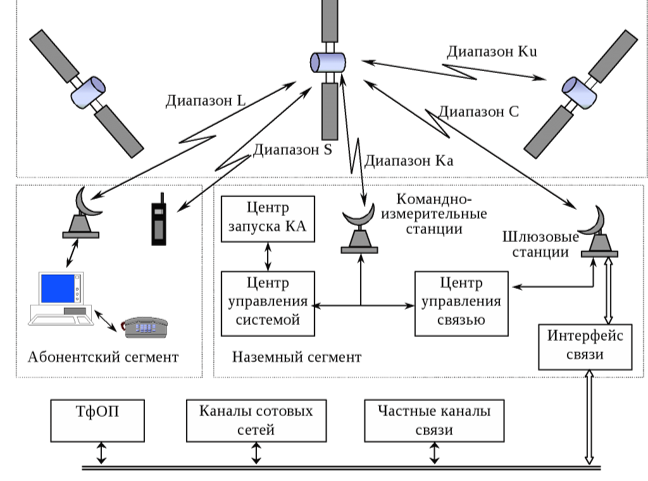
\includegraphics[width=\textwidth]{imgs/1}
    \end{center}
\end{figure}

\subsection{Классификация спутниковых систем связи} 

По виду спутниковой службы: фиксированные, подвижные, вещательные.

Фиксированная спутниковая служба (fixed-satellite service) использует ЗС с заданным местоположением и один или несколько КА. Заданное местоположение может представлять собой определенный фиксированный пункт, расположенный в определенной зоне. В некоторых случаях эта служба включает МЛС: «КА-КА».

Подвижная спутниковая служба (mobile satellite service)  обеспечивает радиосвязь между подвижными ЗС и одной или несколькими РТР, включая МЛС.

В радиовещательной спутниковой службе (broadcasting satellite service) сигналы, ретранслируемые космическими РТР, предназначены для непосредственного приема населением. При этом непосредственным считается как индивидуальный, так и коллективный прием, при котором программы вещания доставляются абонентам с помощью той или иной наземной системы распределения.

Классификация по виду передаваемой информации: многофункциональные, специализированные (радиовещательные, навигационные, передачи данных, в т.ч. спутники ДЗЗ, связные и т.п.). Эта грань в настоящее время стирается путём применения цифровых каналов передачи.

по обслуживаемой территории:

\begin{itemize}
    \item глобальные ССС (Irirdium, Гонец);
    \item региональные системы спутниковой связи (КА Anik-F2 и Taicom-4);
    \item национальные системы спутниковой связи (КА Экспресс);
    \item ведомственные (и специальные) ССС (КА Ямал);
    \item международные и национальные ССС (глобальные, со всемирным охватом, такие как Intelsat, Inmarsat, Irirdium, GlobalStar, Thuraya).
\end{itemize}

по виду передаваемой информации:

Многофункциональные ССС ― VSAT, фактически предоставление канала связи.

Специализированные ССС: передача голоса, служебной информации и т.п. С появлением цифровых каналов связи классификация ССС по виду передаваемой информации  утрачивает своё значение.

По обслуживаемой территории: глобальные, региональные, ведомственные.

По назначению: связные, навигационные, метеорологические, дистанционного зондирования Земли.

\section{Космический сегмент. Орбиты КА космического сегмента спутниковой связи. Недостатки и достоинства орбит связных космических аппаратов.}

Космические системы связи используют следующие орбиты:

\begin{itemize}
    \item геостационарные орбиты (ГСО) КА;
    \item высокоэллиптические орбиты (ВЭО) КА ;
    \item низкие орбиты (НКСС) КА.
\end{itemize}


ГСО используются для создания региональных и глобальных ССС. Пример - КА типа «Ямал», «Экспресс-АМ», «Anik-F2», «Тайком-4» и др., в том числе и военные системы связи Milstar, AENF, DSCS-III  и др.

ВЭО, в основном, используется для обслуживания полярных областей: «Молния-1», Milstar UFO (наклонение к плоскости орбиты 63,4°,  высота апогея, расположенного в северном полушарии, равна 39500 км, высота перигея – 650 км).

\begin{figure}[H]
    \begin{center}
        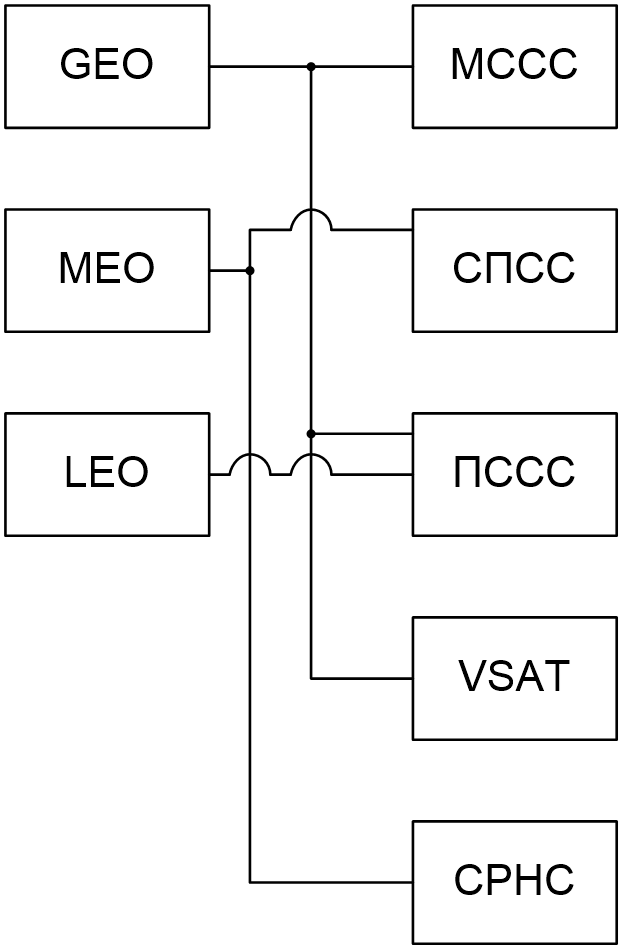
\includegraphics[width=\textwidth/2]{imgs/2}
    \end{center}
\end{figure}

МССС ― магистральная система спутниковой связи; СПСС ―
система подвижной спутниковой связи; ПССС ― персональная система спутниковой связи; СРНС ― спутниковая радионавигационная система. 

\begin{itemize}
    \item GEO – Global Earth Orbit, геостационарная орбита (ГСО): 36000 км;
    \item MEO – Middle Earth Orbit, средневысотная орбита: 10000-20000 км;
    \item LEO – Low Earth Orbit, низкая орбита: 700-1500 км;
    \item Солнечно-синхронная орбита ― дистанцион-ное зондирование земной поверхности;
    \item Высокоэллиптическая орбита, обслуживание полярных регионов, Крайнего Севера и Арктики, региональная ретрансляция ТВ.
\end{itemize}

Солнечно-синхронная орбита (иногда именуемая гелио-синхронной) — геоцентрическая орбита с такими параметрами, что КА, находящийся на ней, проходит над любой точкой земной поверхности приблизительно в одно и то же местное солнечное время. Таким образом, угол освещения земной поверхности будет приблизительно одинаковым на всех проходах КА.

Такие постоянные условия освещения очень хорошо подходят для КА, фотографирующих земную поверхность (в том числе КА дистанционного зондирования земли (ДЗЗ), метеоспутников). 

Однако присутствуют годовые колебания солнечного времени, вызванные эллиптичностью земной орбиты. Например, КА LandSat-7, находящийся на солнечно-синхронной орбите, может пересекать экватор пятнадцать раз в сутки, каждый раз в 10:00 местного времени.

Для достижения подобных характеристик параметры выбираются таким образом, чтобы орбита прецессировала в восточном направлении на 360° в год (приблизительно на 1° в день), компенсируя вращение Земли вокруг Солнца. Прецессия происходит за счёт взаимодействия КА с Землёй, несферичной из-за полярного сжатия. Скорость прецессии зависит от наклонения орбиты.

Нужной скорости прецессии можно достичь лишь для определённого диапазона высот орбит (как правило, выбираются значения 600-800 км, с периодами 96-100мин.), необходимое наклонение для упомянутого диапазона высот около 98°.

Для орбит с большими высотами требуются весьма большие значения наклонения, из-за чего в обслуживаемую зону КА перестают попадать полярные области. Данный тип орбит может иметь различные вариации.

Хотя КА на круговой солнечно-синхронной орбите пересекает экватор в одно и то же местное время, это происходит в разных точках экватора (на разной долготе) из-за того, что Земля поворачивается на некоторый угол между проходами спутника. Предположим, период обращения составляет 96 мин. Это значение нацело делит солнечные сутки на пятнадцать. Таким образом, за сутки спутник пройдёт над пятнадцатью разными точками экватора на дневной стороне орбиты (и еще над пятнадцатью — на ночной), через сутки вернувшись к первой точке. Подбором более сложных (нецелых) отношений, число посещаемых точек может быть увеличено за счёт увеличения периода посещения одной и той же точки.

НКСС применяется для мгновенного охвата ССС всей поверхности Земли. Пример: подвижная спутниковая служба (ПСС) Иридиум и мобильная информационная система связи Гонец (нереальное время).    

Несмотря на широкое применение низко- и средневысотных орбит, самыми надежными считаются системы связи с КА, базирующимися на ГСО. Кроме того, такие системы связи имеют лучшие ТТХ.

\section{Понятие о транспондере или стволе системы спутниковой связи. Структура спутниковой системы связи. Технические характеристики системы спутниковой связи.}

Устройство, принимающее, усиливающее и передающее далее сигнал на той же или другой частоте в соответствии с частотным планом (дуплекс, полудуплекс, частотный дуплекс, временной дуплекс). Стволом РТР или стволом ССС, называется приемопередающий тракт, в котором радиосигналы проходят через общие усилительные элементы (общий передатчик) в некоторой выделенной стволу общей полосе частот. Считается, что:
\begin{itemize}
    \item обычное число стволов 6-12;
    \item число стволов 24-48 на наиболее мощных ИСЗ;
    \item ширина рабочих частот ствола 27-36, 72-120 МГц.
\end{itemize}

Обычно реализуются на ЛБВ либо на твёрдотельных усилителей. Пропускная способность в Мбит/с примерно равна полосе в МГц.

Спутниковая линия – линия связи между ЗС с помощью одного РТР – на каждом направлении включает в себя участок «Земля-спутник» («линия вверх») и участок «спутник-Земля» («линия вниз»)

Линия связи «ЗС-РТР-ЗС» называется скачок, которую обеспечивает станция подскока.

\begin{figure}[H]
    \begin{center}
        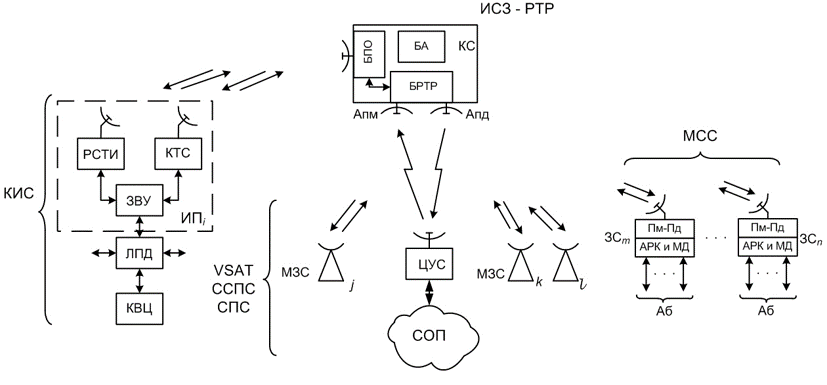
\includegraphics[width=\textwidth]{imgs/3}
    \end{center}
\end{figure}

СОП ― сеть общего пользования; МЗС ― малая земная станция; МСС ― магистральная ССС; КВЦ ― координационно-вычислительный центр; РСТИ ― радиосистема траекторных измерений; ЛПД ― линия передачи данных; КТС ― командно-телеметрическая система; ЗВУ ― звенья системы управления: БПО ― бортовой приёмоответчик.

ЦУСС  ― орган, осуществляющий руководство эксплуатацией системы и ее развитием, т.е. вводом в действие новых ЗС и ИСЗ, расписанием их работы, предоставлением стволов потребителям, проведением ремонтно-профилактических работ и т.п. Центр управления обычно соединяют со станциями сети каналами служебной связи. Иногда центр может совмещаться с передающей станцией системы спутникового вещания либо с контрольной ЗС.

Контрольно-измерительная станция (КИС): 
\begin{itemize}
    \item контроль режима работы ретранслятора космической станции;
    \item определение параметров орбиты ИСЗ;
    \item контроль за соблюдением ЗС сети важных для работы всей сети показателей ― излучаемой мощности, частоты передачи, поляризации, качества модулирующего сигнала и т.п.; 
\end{itemize}

КИС играют важную роль в поддержании нормальной работы системы. КИС бывает универсальной ― работает по многом космическим объектам и специализированная. Часто функции контрольной станции возлагаются на одну из передающих или приемопередающих ЗС сети – центральную ЗС (ЦЗС).

\textbf{Технические характеристики системы спутниковой связи}
\begin{itemize}
    \item Характеристики системы в целом;
    \item Характеристики ретранслятора;
    \item Характеристики земных станций.
    
\end{itemize}

\textbf{Основные показатели систем спутниковой связи}

\begin{itemize}
    \item Зона обслуживания системы;
    \item Пропускная способность системы;
    \item Число и размещение ЗС;
    \item Число ИСЗ и тип их орбиты; 
    \item Точка размещения на геостационарной орбите.
\end{itemize}

\section{Основное противоречие в развитии системы спутниковой связи. Структура бортового космического ретранслятора с комплексом «МЛА-МБЦП».}


\end{document}